\documentclass[aspectratio=169]{beamer}
\usetheme{Madrid}
\usecolortheme{default}

% Packages
\usepackage[utf8]{inputenc}
\usepackage[english]{babel}
\usepackage{graphicx}
\usepackage{tikz}
\usepackage{listings}
\usepackage{booktabs}
\usepackage{array}
\usepackage{colortbl}
\usepackage{xcolor}

% SQL listing configuration
\lstdefinestyle{sqlstyle}{
	language=SQL,
	basicstyle=\ttfamily\small,
	keywordstyle=\color{blue}\bfseries,
	commentstyle=\color{gray}\itshape,
	stringstyle=\color{red},
	showstringspaces=false,
	breaklines=true,
	frame=single,
	numbers=left,
	numberstyle=\tiny\color{gray},
	backgroundcolor=\color{gray!10}
}

\lstset{style=sqlstyle}

% Custom colors
\definecolor{mainblue}{RGB}{0,102,204}
\definecolor{lightblue}{RGB}{173,216,230}
\definecolor{darkgreen}{RGB}{0,128,0}

% Presentation information
\title{Query Language and Groupings}
\subtitle{Aggregate Operators and SQL Clauses}
\author{Computer Science - IIS Fermi Sacconi Ceci}
\date{All rights reserved}
\institute{Ascoli Piceno}

\begin{document}
	
	% Slide 1 - Title
	\begin{frame}
		\titlepage
	\end{frame}
	
	% Slide 2 - Table of Contents
	\begin{frame}{Table of Contents}
		\begin{center}
			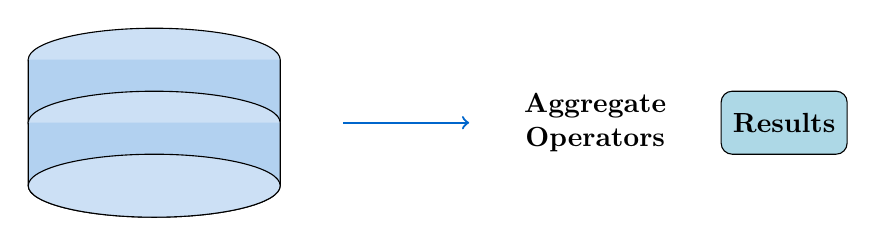
\begin{tikzpicture}[scale=0.8]
				% Database icon
				\draw[fill=mainblue!20] (0,0) ellipse (2cm and 0.5cm);
				\draw[fill=mainblue!30] (-2,0) -- (-2,-1) arc (180:360:2cm and 0.5cm) -- (2,0);
				\draw[fill=mainblue!20] (0,-1) ellipse (2cm and 0.5cm);
				\draw[fill=mainblue!30] (-2,-1) -- (-2,-2) arc (180:360:2cm and 0.5cm) -- (2,-1);
				\draw[fill=mainblue!20] (0,-2) ellipse (2cm and 0.5cm);
				
				% Query arrows
				\draw[->,thick,mainblue] (3,-1) -- (5,-1);
				\node[align=center] at (7,-1) {\textbf{Aggregate}\\\textbf{Operators}};
				
				% Results
				\draw[fill=lightblue,rounded corners] (9,-1.5) rectangle (11,-0.5);
				\node at (10,-1) {\textbf{Results}};
			\end{tikzpicture}
		\end{center}
		
		\begin{itemize}
			\item Aggregate Operators
			\item GROUP BY Clause
			\item HAVING Clause
			\item Result Limitation
		\end{itemize}
	\end{frame}
	
	% Slide 3 - Introduction to aggregate operators
	\begin{frame}{Aggregate Operators}
		\begin{block}{SQL Extension}
			Compared to relational algebra, the most important extension introduced by SQL is that of \textbf{aggregate operators}.
		\end{block}
		
		\vspace{0.3cm}
		
		\textbf{Main characteristics:}
		\begin{itemize}
			\item Aggregate multiple table rows
			\item Perform operations at \emph{relation} level, not tuple level
			\item Return a \textbf{single aggregate value}
			\item Do not select a subset of rows, but calculate values
		\end{itemize}
	\end{frame}
	
	% Slide 4 - Aggregation operations
	\begin{frame}{Aggregate Operators}
		\begin{block}{Functionality}
			Aggregation operations allow you to:
			\begin{itemize}
				\item \textbf{Group} tuples
				\item Perform \textbf{specific calculations} (sums, counts, statistics)
				\item \textbf{Divide} the table into subsets
				\item Group tuples with \textbf{same values} for specific attributes
			\end{itemize}
		\end{block}
		
		\vspace{0.3cm}
		
		\begin{center}
			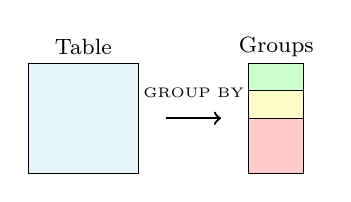
\begin{tikzpicture}[scale=0.7]
				% Original table
				\draw[fill=lightblue!30] (0,0) rectangle (2,2);
				\node at (1,2.3) {\footnotesize Table};
				
				% Arrow
				\draw[->,thick] (2.5,1) -- (3.5,1);
				\node[above] at (3,1.2) {\tiny GROUP BY};
				
				% Groups
				\draw[fill=green!20] (4,1.5) rectangle (5,2);
				\draw[fill=yellow!20] (4,1) rectangle (5,1.5);
				\draw[fill=red!20] (4,0) rectangle (5,1);
				\node at (4.5,2.3) {\footnotesize Groups};
			\end{tikzpicture}
		\end{center}
	\end{frame}
	
	% Slide 5 - Operator characteristics
	\begin{frame}{Aggregate Operators}
		\begin{alertblock}{Fundamental difference}
			Aggregation operators, unlike mathematical operators that act only on the tuple being processed:
		\end{alertblock}
		
		\vspace{0.3cm}
		
		\textbf{Can be applied to multiple tuples} of the table and are characterized by:
		\begin{itemize}
			\item Returning a \textbf{unique value}
			\item Operating on a \textbf{group of values}
			\item Working on values that form a \textbf{column}
		\end{itemize}
		
		\vspace{0.3cm}
		
		\begin{center}
			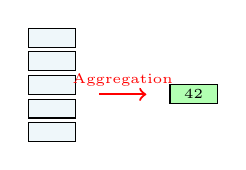
\begin{tikzpicture}[scale=0.6]
				\foreach \y in {0,0.5,1,1.5,2} {
					\draw[fill=lightblue!20] (0,\y) rectangle (1,\y+0.4);
				}
				\draw[->,thick,red] (1.5,1) -- (2.5,1);
				\node[red] at (2,1.3) {\tiny Aggregation};
				\draw[fill=green!30] (3,0.8) rectangle (4,1.2);
				\node at (3.5,1) {\tiny 42};
			\end{tikzpicture}
		\end{center}
	\end{frame}
	
	% Slide 6 - List of operators
	\begin{frame}[fragile]{Aggregate Operators}
		\begin{block}{Main aggregation operators}
			\begin{description}
				\item[\texttt{AVG(field)}] Calculates the \textbf{arithmetic mean}
				\item[\texttt{COUNT(expr|*)}] \textbf{Counts} rows
				\item[\texttt{MAX(expr)}] Calculates the \textbf{maximum} value
				\item[\texttt{MIN(expr)}] Calculates the \textbf{minimum} value
				\item[\texttt{SUM(field)}] Calculates the \textbf{total sum}
				\item[\texttt{STDDEV(field)}] Calculates the \textbf{standard deviation}
			\end{description}
		\end{block}
		
		\vspace{0.2cm}
		
		\begin{center}
			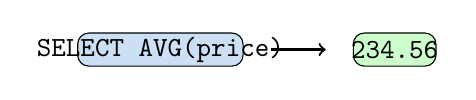
\begin{tikzpicture}[scale=0.7]
				\draw[fill=mainblue!20,rounded corners] (0,0) rectangle (3,0.6);
				\node at (1.5,0.3) {\texttt{SELECT AVG(price)}};
				\draw[->,thick] (3.5,0.3) -- (4.5,0.3);
				\draw[fill=green!20,rounded corners] (5,0) rectangle (6.5,0.6);
				\node at (5.75,0.3) {\texttt{234.56}};
			\end{tikzpicture}
		\end{center}
	\end{frame}
	
	% Slide 7 - GROUP BY and positioning
	\begin{frame}[fragile]{Aggregate Operators}
		\begin{block}{GROUP BY Clause}
			Specifies which fields to perform groupings on.
		\end{block}
		
		\vspace{0.3cm}
		
		\begin{alertblock}{Important}
			Aggregate operators can only appear after these clauses:
			\begin{itemize}
				\item \texttt{SELECT}
				\item \texttt{HAVING}
			\end{itemize}
		\end{alertblock}
		
		\vspace{0.3cm}
		
		\begin{lstlisting}
			SELECT category, COUNT(*) AS number
			FROM products
			GROUP BY category;
		\end{lstlisting}
	\end{frame}
	
	% Slide 8 - HAVING clause
	\begin{frame}[fragile]{The HAVING Clause}
		\begin{block}{How it works}
			The \texttt{HAVING} clause allows you to insert a constraint on the data resulting from the \texttt{GROUP BY} grouping operation.
		\end{block}
		
		\vspace{0.3cm}
		
		\textbf{Difference with WHERE:}
		\begin{itemize}
			\item \texttt{WHERE} operates on \textbf{database fields} (before grouping)
			\item \texttt{HAVING} operates on \textbf{fields resulting from groupings} (after)
		\end{itemize}
		
		\vspace{0.3cm}
		
		\begin{lstlisting}
			SELECT department, AVG(salary) AS average
			FROM employees
			GROUP BY department
			HAVING AVG(salary) > 30000;
		\end{lstlisting}
	\end{frame}
	
	% Slide 9 - COUNT operator
	\begin{frame}[fragile]{COUNT Operator}
		\begin{block}{Syntax}
			\texttt{COUNT(expression | *)}
		\end{block}
		
		\vspace{0.3cm}
		
		\begin{lstlisting}
			SELECT COUNT(*) AS total_cars
			FROM cars;
		\end{lstlisting}
		
		\vspace{0.3cm}
		
		\begin{center}
			\begin{tabular}{|c|}
				\hline
				\rowcolor{lightblue}
				\textbf{total\_cars} \\
				\hline
				12 \\
				\hline
			\end{tabular}
		\end{center}
		
		\vspace{0.2cm}
		
		\textbf{Note:} \texttt{COUNT(*)} counts all rows, including duplicates.
	\end{frame}
	
	% Slide 10 - COUNT with DISTINCT
	\begin{frame}[fragile]{COUNT Operator}
		\begin{block}{Result}
			The result is \textbf{12}: all records that make up the table and are not NULL are counted, regardless of their content.
		\end{block}
		
		\vspace{0.2cm}
		
		\begin{alertblock}{Important}
			\texttt{COUNT} is the only aggregation operator that considers null values in the calculation.
		\end{alertblock}
		
		\vspace{0.2cm}
		
		\textbf{To count distinct values:}
		\begin{lstlisting}
			SELECT COUNT(DISTINCT brand) AS different_brands
			FROM cars;
		\end{lstlisting}
		
		\begin{center}
			\begin{tabular}{|c|}
				\hline
				\rowcolor{lightblue}
				\textbf{different\_brands} \\
				\hline
				8 \\
				\hline
			\end{tabular}
		\end{center}
	\end{frame}
	
	% Slide 11 - AVG operator
	\begin{frame}[fragile]{AVG Operator}
		\begin{block}{Arithmetic Mean}
			Calculates the average of values in a numeric column.
		\end{block}
		
		\vspace{0.3cm}
		
		\begin{lstlisting}
			SELECT AVG(price) AS average_price
			FROM cars;
		\end{lstlisting}
		
		\vspace{0.3cm}
		
		\begin{center}
			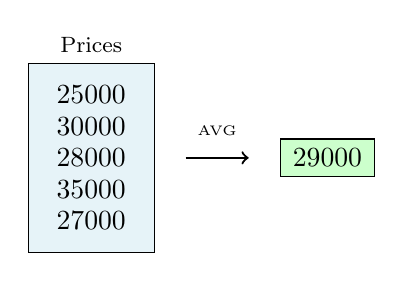
\begin{tikzpicture}[scale=0.8]
				% Input table
				\draw[fill=lightblue!30] (0,0) rectangle (2,3);
				\node at (1,3.3) {\footnotesize Prices};
				\node at (1,2.5) {25000};
				\node at (1,2) {30000};
				\node at (1,1.5) {28000};
				\node at (1,1) {35000};
				\node at (1,0.5) {27000};
				
				% Arrow
				\draw[->,thick] (2.5,1.5) -- (3.5,1.5);
				\node[above] at (3,1.7) {\tiny AVG};
				
				% Result
				\draw[fill=green!20] (4,1.2) rectangle (5.5,1.8);
				\node at (4.75,1.5) {29000};
			\end{tikzpicture}
		\end{center}
	\end{frame}
	
	% Slide 12 - MIN and MAX operators intro
	\begin{frame}[fragile]{MIN and MAX Operators}
		\begin{block}{How they work}
			\texttt{MAX} and \texttt{MIN} return the highest and lowest values contained within a column.
		\end{block}
		
		\vspace{0.3cm}
		
		\textbf{Behavior by data type:}
		\begin{itemize}
			\item \textbf{Numeric fields:} returns the numeric value
			\item \textbf{Text fields:} identifies the field that, in alphabetical order, is last (MAX) or first (MIN)
			\item Ordering according to the \textbf{ASCII} code table
			\item \textbf{Lexicographic} ordering
		\end{itemize}
		
		\vspace{0.3cm}
		
		\begin{center}
			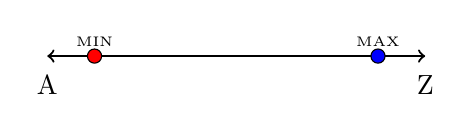
\begin{tikzpicture}[scale=0.6]
				\draw[<->,thick] (0,0) -- (8,0);
				\node[below] at (0,-0.2) {A};
				\node[below] at (8,-0.2) {Z};
				\draw[fill=red] (1,0) circle (0.15) node[above] {\tiny MIN};
				\draw[fill=blue] (7,0) circle (0.15) node[above] {\tiny MAX};
			\end{tikzpicture}
		\end{center}
	\end{frame}
	
	% Slide 13 - MIN and MAX with expressions
	\begin{frame}[fragile]{MIN and MAX Operators}
		\begin{block}{Mathematical expressions}
			It is possible to use mathematical expressions as arguments for the \texttt{MIN} and \texttt{MAX} operators.
		\end{block}
		
		\vspace{0.3cm}
		
		\begin{lstlisting}
			SELECT MAX(price * 1.22) AS max_price_vat
			FROM cars;
		\end{lstlisting}
		
		\vspace{0.3cm}
		
		\begin{lstlisting}
			SELECT MIN(price - discount) AS min_price_discounted
			FROM cars;
		\end{lstlisting}
		
		\vspace{0.3cm}
		
		\begin{center}
			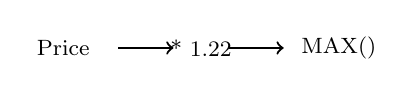
\begin{tikzpicture}[scale=0.7]
				\node at (0,0.5) {\footnotesize Price};
				\draw[->,thick] (1,0.5) -- (2,0.5);
				\node at (2.5,0.5) {\footnotesize * 1.22};
				\draw[->,thick] (3,0.5) -- (4,0.5);
				\node at (5,0.5) {\footnotesize MAX()};
			\end{tikzpicture}
		\end{center}
	\end{frame}
	
	% Slide 14 - MIN example
	\begin{frame}[fragile]{MIN and MAX Operators}
		\begin{lstlisting}
			SELECT MIN(salary) AS minimum_salary
			FROM employees;
		\end{lstlisting}
		
		\vspace{0.3cm}
		
		\begin{center}
			\begin{tabular}{|l|c|}
				\hline
				\rowcolor{lightblue}
				\textbf{Name} & \textbf{Salary} \\
				\hline
				Mario Rossi & 28000 \\
				Laura Bianchi & 32000 \\
				Giuseppe Verdi & \cellcolor{yellow}\textbf{25000} \\
				Anna Neri & 35000 \\
				\hline
			\end{tabular}
			
			\vspace{0.5cm}
			
			\begin{tabular}{|c|}
				\hline
				\rowcolor{green!30}
				\textbf{minimum\_salary} \\
				\hline
				\textbf{25000} \\
				\hline
			\end{tabular}
		\end{center}
	\end{frame}
	
	% Slide 15 - MAX example
	\begin{frame}[fragile]{MIN and MAX Operators}
		\begin{lstlisting}
			SELECT MAX(salary) AS maximum_salary
			FROM employees;
		\end{lstlisting}
		
		\vspace{0.3cm}
		
		\begin{center}
			\begin{tabular}{|l|c|}
				\hline
				\rowcolor{lightblue}
				\textbf{Name} & \textbf{Salary} \\
				\hline
				Mario Rossi & 28000 \\
				Laura Bianchi & 32000 \\
				Giuseppe Verdi & 25000 \\
				Anna Neri & \cellcolor{yellow}\textbf{35000} \\
				\hline
			\end{tabular}
			
			\vspace{0.5cm}
			
			\begin{tabular}{|c|}
				\hline
				\rowcolor{green!30}
				\textbf{maximum\_salary} \\
				\hline
				\textbf{35000} \\
				\hline
			\end{tabular}
		\end{center}
	\end{frame}
	
	% Slide 16 - MAX on text fields
	\begin{frame}[fragile]{MIN and MAX Operators}
		\begin{lstlisting}
			SELECT MAX(surname) AS max_surname
			FROM employees;
		\end{lstlisting}
		
		\vspace{0.3cm}
		
		\begin{center}
			\begin{tabular}{|l|}
				\hline
				\rowcolor{lightblue}
				\textbf{Surname} \\
				\hline
				Bianchi \\
				Neri \\
				Rossi \\
				\cellcolor{yellow}\textbf{Verdi} \\
				\hline
			\end{tabular}
			
			\vspace{0.5cm}
			
			\begin{tabular}{|c|}
				\hline
				\rowcolor{green!30}
				\textbf{max\_surname} \\
				\hline
				\textbf{Verdi} \\
				\hline
			\end{tabular}
		\end{center}
		
		\vspace{0.2cm}
		\footnotesize{Alphabetical order: B < N < R < V}
	\end{frame}
	
	% Slide 17 - MIN on text fields
	\begin{frame}[fragile]{MIN and MAX Operators}
		\begin{lstlisting}
			SELECT MIN(surname) AS min_surname
			FROM employees;
		\end{lstlisting}
		
		\vspace{0.3cm}
		
		\begin{center}
			\begin{tabular}{|l|}
				\hline
				\rowcolor{lightblue}
				\textbf{Surname} \\
				\hline
				\cellcolor{yellow}\textbf{Bianchi} \\
				Neri \\
				Rossi \\
				Verdi \\
				\hline
			\end{tabular}
			
			\vspace{0.5cm}
			
			\begin{tabular}{|c|}
				\hline
				\rowcolor{green!30}
				\textbf{min\_surname} \\
				\hline
				\textbf{Bianchi} \\
				\hline
			\end{tabular}
		\end{center}
		
		\vspace{0.2cm}
		\footnotesize{Alphabetical order: B < N < R < V}
	\end{frame}
	
	% Slide 18 - Complex expressions
	\begin{frame}[fragile]{MIN and MAX Operators}
		\begin{block}{Complex expressions}
			Let's see how to apply arithmetic operators in the query. To know the difference between minimum and maximum employee salaries, expressed as a percentage:
		\end{block}
		
		\vspace{0.3cm}
		
		\begin{lstlisting}
			SELECT 
			(MAX(salary) - MIN(salary)) / 
			MAX(salary) * 100 AS percentage_diff
			FROM employees;
		\end{lstlisting}
		
		\vspace{0.3cm}
		
		\begin{center}
			\begin{tabular}{|c|}
				\hline
				\rowcolor{green!30}
				\textbf{percentage\_diff} \\
				\hline
				28.57 \\
				\hline
			\end{tabular}
		\end{center}
		
		\footnotesize{The difference between maximum and minimum salary is 28.57\%}
	\end{frame}
	
	% Slide 19 - SUM operator intro
	\begin{frame}[fragile]{SUM Operator}
		\begin{block}{Total sum}
			Calculates the sum of all values in a numeric column.
		\end{block}
		
		\vspace{0.3cm}
		
		\begin{lstlisting}
			SELECT SUM(salary) AS total_salaries
			FROM employees;
		\end{lstlisting}
		
		\vspace{0.3cm}
		
		\begin{center}
			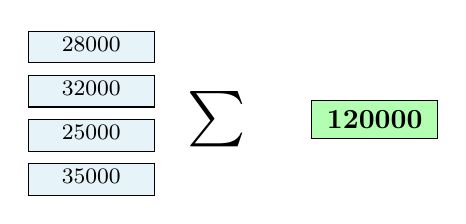
\begin{tikzpicture}[scale=0.8]
				% Values
				\foreach \y/\val in {3/28000, 2.3/32000, 1.6/25000, 0.9/35000} {
					\draw[fill=lightblue!30] (0,\y-0.3) rectangle (2,\y+0.2);
					\node at (1,\y) {\footnotesize \val};
				}
				
				% Sum symbol
				\node[scale=2] at (3,1.8) {$\sum$};
				
				% Result
				\draw[fill=green!30] (4.5,1.5) rectangle (6.5,2.1);
				\node at (5.5,1.8) {\textbf{120000}};
			\end{tikzpicture}
		\end{center}
	\end{frame}
	
	% Slide 20 - SUM example
	\begin{frame}[fragile]{SUM Operator}
		\begin{lstlisting}
			SELECT 
			SUM(amount) AS total_sales,
			SUM(quantity) AS total_pieces
			FROM sales
			WHERE year = 2024;
		\end{lstlisting}
		
		\vspace{0.3cm}
		
		\begin{center}
			\begin{tabular}{|c|c|}
				\hline
				\rowcolor{lightblue}
				\textbf{total\_sales} & \textbf{total\_pieces} \\
				\hline
				158750.50 & 1243 \\
				\hline
			\end{tabular}
		\end{center}
		
		\vspace{0.3cm}
		
		\begin{alertblock}{Note}
			\texttt{SUM} ignores NULL values in the calculation.
		\end{alertblock}
	\end{frame}
	
	% Slide 21 - AVG and STDDEV
	\begin{frame}[fragile]{AVG and STDDEV Operators}
		\begin{lstlisting}
			SELECT 
			AVG(salary) AS average_salary,
			STDDEV(salary) AS standard_deviation
			FROM employees;
		\end{lstlisting}
		
		\vspace{0.3cm}
		
		\begin{center}
			\begin{tabular}{|c|c|}
				\hline
				\rowcolor{lightblue}
				\textbf{average\_salary} & \textbf{standard\_deviation} \\
				\hline
				30000.00 & 4082.48 \\
				\hline
			\end{tabular}
		\end{center}
		
		\vspace{0.3cm}
		
		\begin{center}
			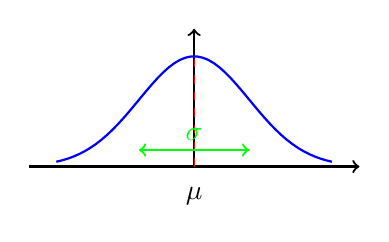
\begin{tikzpicture}[scale=0.7]
				% Simplified Gaussian curve
				\draw[->,thick] (-3,0) -- (3,0);
				\draw[->,thick] (0,0) -- (0,2.5);
				\draw[blue,thick,domain=-2.5:2.5,samples=50] plot (\x,{2*exp(-\x*\x/2)});
				\draw[dashed,red] (0,0) -- (0,2);
				\node[below] at (0,-0.2) {$\mu$};
				\draw[<->,green,thick] (-1,0.3) -- (1,0.3);
				\node[above,green] at (0,0.3) {$\sigma$};
			\end{tikzpicture}
		\end{center}
	\end{frame}
	
	% Slide 22 - GROUP BY syntax
	\begin{frame}[fragile]{The GROUP BY Clause}
		\begin{block}{Function}
			The \texttt{GROUP BY} clause is used to group and process uniformly different rows that have equal values in a specific column in the source table.
		\end{block}
		
		\vspace{0.3cm}
		
		\textbf{Syntax:}
		\begin{lstlisting}
			SELECT column1, aggregate_function(column2)
			FROM table
			WHERE condition
			GROUP BY column1;
		\end{lstlisting}
		
		\vspace{0.3cm}
		
		\begin{center}
			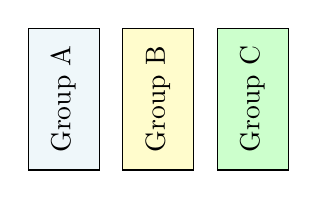
\begin{tikzpicture}[scale=0.6]
				\draw[fill=lightblue!20] (0,0) rectangle (1.5,3);
				\node[rotate=90] at (0.75,1.5) {Group A};
				\draw[fill=yellow!20] (2,0) rectangle (3.5,3);
				\node[rotate=90] at (2.75,1.5) {Group B};
				\draw[fill=green!20] (4,0) rectangle (5.5,3);
				\node[rotate=90] at (4.75,1.5) {Group C};
			\end{tikzpicture}
		\end{center}
	\end{frame}
	
	% Slide 23 - Execution priority 1
	\begin{frame}{The GROUP BY Clause}
		\begin{block}{Execution order}
			Taking into account the following considerations, let's clarify the priorities during the execution of a selection with grouping.
		\end{block}
		
		\vspace{0.3cm}
		
		\textbf{Processing phases:}
		\begin{enumerate}
			\item Execution of the \texttt{JOIN}, if present
			\item Selection on tuples with the condition after \texttt{WHERE}
		\end{enumerate}
		
		\vspace{0.3cm}
		
		\begin{center}
			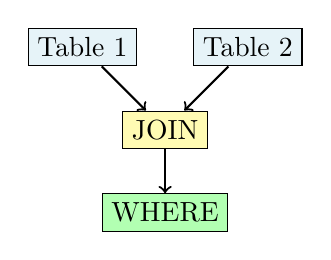
\begin{tikzpicture}[scale=0.7]
				\node[draw,rectangle,fill=lightblue!30] (t1) at (0,2) {Table 1};
				\node[draw,rectangle,fill=lightblue!30] (t2) at (3,2) {Table 2};
				\node[draw,rectangle,fill=yellow!30] (join) at (1.5,0.5) {JOIN};
				\node[draw,rectangle,fill=green!30] (where) at (1.5,-1) {WHERE};
				\draw[->,thick] (t1) -- (join);
				\draw[->,thick] (t2) -- (join);
				\draw[->,thick] (join) -- (where);
			\end{tikzpicture}
		\end{center}
	\end{frame}
	
	% Slide 24 - Execution priority 2
	\begin{frame}[fragile]{The GROUP BY Clause}
		\textbf{Processing phases (continued):}
		\begin{enumerate}
			\setcounter{enumi}{2}
			\item Grouping based on fields specified after \texttt{GROUP BY}
			\item List of values specified after \texttt{SELECT} (target list)
			\item Selection of tuples that satisfy the condition after \texttt{HAVING}
		\end{enumerate}
		
		\vspace{0.3cm}
		
		\begin{center}
			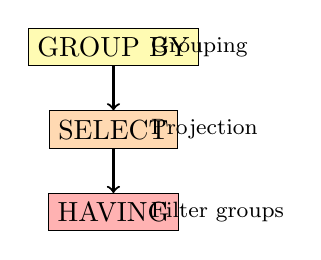
\begin{tikzpicture}[scale=0.7]
				\node[draw,rectangle,fill=yellow!30] (group) at (0,1.5) {GROUP BY};
				\node[draw,rectangle,fill=orange!30] (select) at (0,0) {SELECT};
				\node[draw,rectangle,fill=red!30] (having) at (0,-1.5) {HAVING};
				\draw[->,thick] (group) -- (select);
				\draw[->,thick] (select) -- (having);
				\node[right] at (0.5,1.5) {\footnotesize Grouping};
				\node[right] at (0.5,0) {\footnotesize Projection};
				\node[right] at (0.5,-1.5) {\footnotesize Filter groups};
			\end{tikzpicture}
		\end{center}
	\end{frame}
	
	% Slide 25 - GROUP BY example 1
	\begin{frame}[fragile]{The GROUP BY Clause}
		\begin{lstlisting}
			SELECT department, COUNT(*) AS number_employees
			FROM employees
			GROUP BY department;
		\end{lstlisting}
		
		\vspace{0.3cm}
		
		\begin{center}
			\textbf{Original table:}
			\begin{tabular}{|l|c|}
				\hline
				\rowcolor{lightblue}
				\textbf{Name} & \textbf{Department} \\
				\hline
				Mario & Sales \\
				Laura & IT \\
				Giuseppe & Sales \\
				Anna & IT \\
				Carlo & Marketing \\
				\hline
			\end{tabular}
			
			\vspace{0.3cm}
			
			\textbf{Result:}
			\begin{tabular}{|l|c|}
				\hline
				\rowcolor{green!30}
				\textbf{department} & \textbf{number\_employees} \\
				\hline
				Sales & 2 \\
				IT & 2 \\
				Marketing & 1 \\
				\hline
			\end{tabular}
		\end{center}
	\end{frame}
	
	% Slide 26 - GROUP BY example 2
	\begin{frame}[fragile]{The GROUP BY Clause}
		\begin{lstlisting}
			SELECT category, AVG(price) AS average_price
			FROM products
			GROUP BY category;
		\end{lstlisting}
		
		\vspace{0.3cm}
		
		\begin{center}
			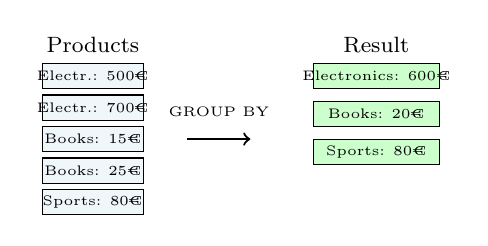
\begin{tikzpicture}[scale=0.8]
				% Original table
				\node at (0,3) {\footnotesize Products};
				\foreach \y/\cat/\pr in {2.5/Electr./500, 2/Electr./700, 1.5/Books/15, 1/Books/25, 0.5/Sports/80} {
					\draw[fill=lightblue!20] (-0.8,\y-0.2) rectangle (0.8,\y+0.2);
					\node[font=\tiny] at (0,\y) {\cat: \pr€};
				}
				
				% Arrow
				\draw[->,thick] (1.5,1.5) -- (2.5,1.5);
				\node[above,font=\tiny] at (2,1.7) {GROUP BY};
				
				% Result
				\node at (4.5,3) {\footnotesize Result};
				\draw[fill=green!20] (3.5,2.3) rectangle (5.5,2.7);
				\node[font=\tiny] at (4.5,2.5) {Electronics: 600€};
				\draw[fill=green!20] (3.5,1.7) rectangle (5.5,2.1);
				\node[font=\tiny] at (4.5,1.9) {Books: 20€};
				\draw[fill=green!20] (3.5,1.1) rectangle (5.5,1.5);
				\node[font=\tiny] at (4.5,1.3) {Sports: 80€};
			\end{tikzpicture}
		\end{center}
	\end{frame}
	
	% Slide 27 - GROUP BY example 3
	\begin{frame}[fragile]{The GROUP BY Clause}
		\begin{lstlisting}
			SELECT 
			year, 
			month, 
			SUM(sales) AS total_sales
			FROM monthly_sales
			GROUP BY year, month
			ORDER BY year, month;
		\end{lstlisting}
		
		\vspace{0.3cm}
		
		\begin{center}
			\begin{tabular}{|c|c|c|}
				\hline
				\rowcolor{lightblue}
				\textbf{year} & \textbf{month} & \textbf{total\_sales} \\
				\hline
				2023 & 1 & 45000 \\
				2023 & 2 & 52000 \\
				2024 & 1 & 48000 \\
				2024 & 2 & 55000 \\
				\hline
			\end{tabular}
		\end{center}
		
		\vspace{0.2cm}
		\footnotesize{Grouping on \textbf{multiple columns}}
	\end{frame}
	
	% Slide 28 - GROUP BY example 4
	\begin{frame}[fragile]{The GROUP BY Clause}
		\begin{lstlisting}
			SELECT 
			city,
			COUNT(*) AS number_customers,
			SUM(orders) AS total_orders
			FROM customers
			GROUP BY city;
		\end{lstlisting}
		
		\vspace{0.3cm}
		
		\begin{center}
			\begin{tabular}{|l|c|c|}
				\hline
				\rowcolor{lightblue}
				\textbf{city} & \textbf{number\_customers} & \textbf{total\_orders} \\
				\hline
				Rome & 15 & 234 \\
				Milan & 22 & 387 \\
				Naples & 8 & 145 \\
				Turin & 12 & 198 \\
				\hline
			\end{tabular}
		\end{center}
	\end{frame}
	
	% Slide 29 - GROUP BY example 5
	\begin{frame}[fragile]{The GROUP BY Clause}
		\begin{lstlisting}
			SELECT 
			brand,
			model,
			COUNT(*) AS units_sold,
			AVG(price) AS average_price
			FROM cars_sold
			GROUP BY brand, model
			ORDER BY units_sold DESC;
		\end{lstlisting}
		
		\vspace{0.3cm}
		
		\begin{center}
			\begin{tabular}{|l|l|c|c|}
				\hline
				\rowcolor{lightblue}
				\textbf{brand} & \textbf{model} & \textbf{units} & \textbf{price} \\
				\hline
				Fiat & Panda & 45 & 12500 \\
				Volkswagen & Golf & 38 & 22000 \\
				Ford & Fiesta & 32 & 15000 \\
				\hline
			\end{tabular}
		\end{center}
	\end{frame}
	
	% Slide 30 - GROUP BY example 6
	\begin{frame}[fragile]{The GROUP BY Clause}
		\begin{lstlisting}
			SELECT 
			YEAR(sale_date) AS year,
			MONTH(sale_date) AS month,
			COUNT(*) AS number_transactions,
			SUM(amount) AS revenue
			FROM transactions
			GROUP BY YEAR(sale_date), MONTH(sale_date);
		\end{lstlisting}
		
		\vspace{0.2cm}
		
		\begin{center}
			\begin{tabular}{|c|c|c|c|}
				\hline
				\rowcolor{lightblue}
				\textbf{year} & \textbf{month} & \textbf{transactions} & \textbf{revenue} \\
				\hline
				2024 & 10 & 152 & 45200.00 \\
				2024 & 11 & 178 & 52800.00 \\
				2024 & 12 & 201 & 68500.00 \\
				\hline
			\end{tabular}
		\end{center}
		
		\vspace{0.2cm}
		\footnotesize{Grouping with \textbf{functions} in columns}
	\end{frame}
	
	% Slide 31 - HAVING example 1
	\begin{frame}[fragile]{The HAVING Clause}
		\begin{lstlisting}
			SELECT department, AVG(salary) AS average_salary
			FROM employees
			GROUP BY department
			HAVING AVG(salary) > 30000;
		\end{lstlisting}
		
		\vspace{0.3cm}
		
		\begin{center}
			\textbf{All groups:}
			\begin{tabular}{|l|c|}
				\hline
				\rowcolor{lightblue}
				\textbf{department} & \textbf{average\_salary} \\
				\hline
				Sales & 28000 \\
				IT & \cellcolor{yellow}35000 \\
				Marketing & 27000 \\
				Production & \cellcolor{yellow}32000 \\
				\hline
			\end{tabular}
			
			\vspace{0.3cm}
			
			\textbf{Result with HAVING:}
			\begin{tabular}{|l|c|}
				\hline
				\rowcolor{green!30}
				\textbf{department} & \textbf{average\_salary} \\
				\hline
				IT & 35000 \\
				Production & 32000 \\
				\hline
			\end{tabular}
		\end{center}
	\end{frame}
	
	% Slide 32 - HAVING example 2
	\begin{frame}[fragile]{The HAVING Clause}
		\begin{lstlisting}
			SELECT category, COUNT(*) AS number_products
			FROM products
			GROUP BY category
			HAVING COUNT(*) >= 5;
		\end{lstlisting}
		
		\vspace{0.3cm}
		
		\begin{center}
			\begin{tabular}{|l|c|}
				\hline
				\rowcolor{green!30}
				\textbf{category} & \textbf{number\_products} \\
				\hline
				Electronics & 12 \\
				Clothing & 8 \\
				Home & 6 \\
				\hline
			\end{tabular}
		\end{center}
		
		\vspace{0.3cm}
		
		\begin{alertblock}{Note}
			\texttt{HAVING} filters groups \textbf{after} aggregation, while \texttt{WHERE} filters rows \textbf{before}.
		\end{alertblock}
	\end{frame}
	
	% Slide 33 - HAVING example 3
	\begin{frame}[fragile]{The HAVING Clause}
		\begin{lstlisting}
			SELECT 
			customer_id,
			SUM(amount) AS total_purchases
			FROM orders
			WHERE year = 2024
			GROUP BY customer_id
			HAVING SUM(amount) > 10000;
		\end{lstlisting}
		
		\vspace{0.3cm}
		
		\begin{center}
			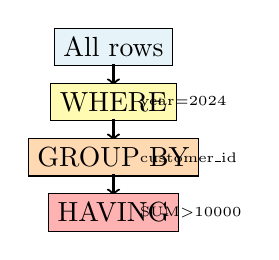
\begin{tikzpicture}[scale=0.7]
				\node[draw,rectangle,fill=lightblue!30] at (0,3) {All rows};
				\draw[->,thick] (0,2.7) -- (0,2.3);
				\node[draw,rectangle,fill=yellow!30] at (0,2) {WHERE};
				\node[right,font=\tiny] at (0.3,2) {year=2024};
				\draw[->,thick] (0,1.7) -- (0,1.3);
				\node[draw,rectangle,fill=orange!30] at (0,1) {GROUP BY};
				\node[right,font=\tiny] at (0.3,1) {customer\_id};
				\draw[->,thick] (0,0.7) -- (0,0.3);
				\node[draw,rectangle,fill=red!30] at (0,0) {HAVING};
				\node[right,font=\tiny] at (0.3,0) {SUM>10000};
			\end{tikzpicture}
		\end{center}
	\end{frame}
	
	% Slide 34 - HAVING example 4
	\begin{frame}[fragile]{The HAVING Clause}
		\begin{lstlisting}
			SELECT 
			city,
			COUNT(*) AS number_orders,
			AVG(amount) AS average_amount
			FROM orders
			GROUP BY city
			HAVING COUNT(*) > 10 AND AVG(amount) > 500;
		\end{lstlisting}
		
		\vspace{0.3cm}
		
		\begin{center}
			\begin{tabular}{|l|c|c|}
				\hline
				\rowcolor{green!30}
				\textbf{city} & \textbf{number\_orders} & \textbf{average\_amount} \\
				\hline
				Milan & 25 & 675.50 \\
				Rome & 18 & 820.30 \\
				\hline
			\end{tabular}
		\end{center}
		
		\vspace{0.2cm}
		\footnotesize{\textbf{Multiple} conditions in HAVING}
	\end{frame}
	
	% Slide 35 - HAVING example 5
	\begin{frame}[fragile]{The HAVING Clause}
		\begin{lstlisting}
			SELECT 
			brand,
			COUNT(*) AS models,
			MIN(price) AS min_price,
			MAX(price) AS max_price
			FROM automobiles
			GROUP BY brand
			HAVING MAX(price) - MIN(price) > 20000;
		\end{lstlisting}
		
		\vspace{0.3cm}
		
		\begin{center}
			\begin{tabular}{|l|c|c|c|}
				\hline
				\rowcolor{green!30}
				\textbf{brand} & \textbf{models} & \textbf{min\_price} & \textbf{max\_price} \\
				\hline
				BMW & 8 & 35000 & 85000 \\
				Mercedes & 6 & 40000 & 95000 \\
				\hline
			\end{tabular}
		\end{center}
		
		\vspace{0.2cm}
		\footnotesize{HAVING with \textbf{expressions} between aggregations}
	\end{frame}
	
	% Slide 36 - LIMIT intro
	\begin{frame}[fragile]{Limiting Result Tuples}
		\begin{block}{LIMIT Clause}
			Allows you to limit the number of rows returned by the query.
		\end{block}
		
		\vspace{0.3cm}
		
		\textbf{Syntax:}
		\begin{lstlisting}
			SELECT columns
			FROM table
			WHERE condition
			ORDER BY column
			LIMIT number;
		\end{lstlisting}
		
		\vspace{0.3cm}
		
		\textbf{Common uses:}
		\begin{itemize}
			\item Display only the first N results
			\item Implement pagination
			\item Optimize query performance
		\end{itemize}
	\end{frame}
	
	% Slide 37 - LIMIT example 1
	\begin{frame}[fragile]{Limiting Result Tuples}
		\begin{lstlisting}
			SELECT name, surname, salary
			FROM employees
			ORDER BY salary DESC
			LIMIT 5;
		\end{lstlisting}
		
		\vspace{0.3cm}
		
		\begin{center}
			\textbf{Top 5 highest salaries:}
			\begin{tabular}{|l|l|c|}
				\hline
				\rowcolor{lightblue}
				\textbf{name} & \textbf{surname} & \textbf{salary} \\
				\hline
				Anna & Neri & 45000 \\
				Mario & Rossi & 42000 \\
				Laura & Bianchi & 38000 \\
				Giuseppe & Verdi & 35000 \\
				Carlo & Gialli & 33000 \\
				\hline
			\end{tabular}
		\end{center}
		
		\vspace{0.2cm}
		\footnotesize{Returns only the first 5 ordered rows}
	\end{frame}
	
	% Slide 38 - LIMIT with OFFSET
	\begin{frame}[fragile]{Limiting Result Tuples}
		\begin{block}{Pagination with OFFSET}
			\texttt{OFFSET} allows you to skip a specified number of rows.
		\end{block}
		
		\vspace{0.3cm}
		
		\begin{lstlisting}
			SELECT name, price
			FROM products
			ORDER BY price DESC
			LIMIT 10 OFFSET 20;
		\end{lstlisting}
		
		\vspace{0.3cm}
		
		\begin{center}
			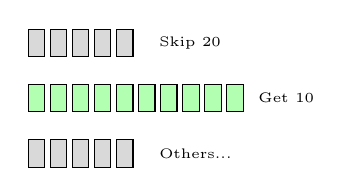
\begin{tikzpicture}[scale=0.7]
				\foreach \x in {0,...,4} {
					\draw[fill=gray!30] (\x*0.4,2) rectangle (\x*0.4+0.3,2.5);
				}
				\node[right] at (2.2,2.25) {\tiny Skip 20};
				
				\foreach \x in {0,...,9} {
					\draw[fill=green!30] (\x*0.4,1) rectangle (\x*0.4+0.3,1.5);
				}
				\node[right] at (4,1.25) {\tiny Get 10};
				
				\foreach \x in {0,...,4} {
					\draw[fill=gray!30] (\x*0.4,0) rectangle (\x*0.4+0.3,0.5);
				}
				\node[right] at (2.2,0.25) {\tiny Others...};
			\end{tikzpicture}
		\end{center}
		
		\vspace{0.2cm}
		\footnotesize{Useful for pagination: page 3 = LIMIT 10 OFFSET 20}
	\end{frame}
	
	% Slide 39 - LIMIT practical example
	\begin{frame}[fragile]{Limiting Result Tuples}
		\begin{lstlisting}
			SELECT 
			product,
			sales,
			revenue
			FROM sales_statistics
			ORDER BY revenue DESC
			LIMIT 3;
		\end{lstlisting}
		
		\vspace{0.3cm}
		
		\begin{center}
			\textbf{Top 3 products by revenue:}
			\begin{tabular}{|l|c|c|}
				\hline
				\rowcolor{lightblue}
				\textbf{product} & \textbf{sales} & \textbf{revenue} \\
				\hline
				\cellcolor{yellow!50}Laptop Pro & 234 & 234000 € \\
				\cellcolor{yellow!30}Smartphone X & 456 & 182400 € \\
				\cellcolor{yellow!10}Tablet Plus & 198 & 99000 € \\
				\hline
			\end{tabular}
		\end{center}
		
		\vspace{0.3cm}
		
		\begin{alertblock}{Best Practice}
			Always use \texttt{ORDER BY} with \texttt{LIMIT} for consistent results.
		\end{alertblock}
	\end{frame}
	
	% Slide 40 - LIMIT and performance
	\begin{frame}[fragile]{Limiting Result Tuples}
		\begin{block}{Advantages of LIMIT}
			\begin{itemize}
				\item \textbf{Performance:} reduces database load
				\item \textbf{Memory:} transfers less data
				\item \textbf{Usability:} improves user experience
				\item \textbf{Testing:} useful for testing queries on large datasets
			\end{itemize}
		\end{block}
		
		\vspace{0.3cm}
		
		\begin{lstlisting}
			-- Test query on large table
			SELECT * FROM event_logs
			WHERE date >= '2024-01-01'
			LIMIT 100;
		\end{lstlisting}
		
		\vspace{0.3cm}
		
		\begin{center}
			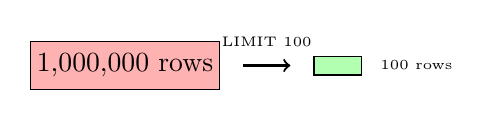
\begin{tikzpicture}[scale=0.6]
				\draw[fill=red!30] (0,0) rectangle (4,1);
				\node at (2,0.5) {1,000,000 rows};
				\draw[->,thick] (4.5,0.5) -- (5.5,0.5);
				\node[above] at (5,0.7) {\tiny LIMIT 100};
				\draw[fill=green!30] (6,0.3) rectangle (7,0.7);
				\node[right] at (7.2,0.5) {\tiny 100 rows};
			\end{tikzpicture}
		\end{center}
	\end{frame}
	
\end{document}